%% Accompanies image file 'ReducTraj5.pdf' (pdf, eps, ps)
%% read dasbuch/book/FigSrc/inkscape/00ReadMe.txt
%% Creator: Inkscape 0.48.0, www.inkscape.org
%% PDF/EPS/PS + LaTeX output extension by Johan Engelen, 2010
%%
%% To include the image in your LaTeX document, write
%%   \input{<filename>.pdf_tex}
%%  instead of
%%   \includegraphics{<filename>.pdf}
%% To scale the image, write
%%   \def\svgwidth{<desired width>}
%%   \input{<filename>.pdf_tex}
%%  instead of
%%   \includegraphics[width=<desired width>]{<filename>.pdf}
%%
%% Images with a different path to the parent latex file can
%% be accessed with the `import' package (which may need to be
%% installed) using
%%   \usepackage{import}
%% in the preamble, and then including the image with
%%   \import{<path to file>}{<filename>.pdf_tex}
%% Alternatively, one can specify
%%   \graphicspath{{<path to file>/}}
%%
%% \unitlength defines the units used in the Picture Environment
%% The default value is 1 point (approximately 1/72 inch)
%%
%% For more information, please see info/svg-inkscape on CTAN:
%%   http://tug.ctan.org/tex-archive/info/svg-inkscape

\begingroup
  \makeatletter
  \providecommand\color[2][]{%
    \errmessage{(Inkscape) Color is used for the text in Inkscape, but the package 'color.sty' is not loaded}
    \renewcommand\color[2][]{}%
  }
  \providecommand\transparent[1]{%
    \errmessage{(Inkscape) Transparency is used (non-zero) for the text in Inkscape, but the package 'transparent.sty' is not loaded}
    \renewcommand\transparent[1]{}%
  }
  \providecommand\rotatebox[2]{#2}
  \ifx\svgwidth\undefined
    \setlength{\unitlength}{382.7pt}
  \else
    \setlength{\unitlength}{\svgwidth}
  \fi
  \global\let\svgwidth\undefined
  \makeatother
  \begin{picture}(1,0.8361641)%
    \put(0,0){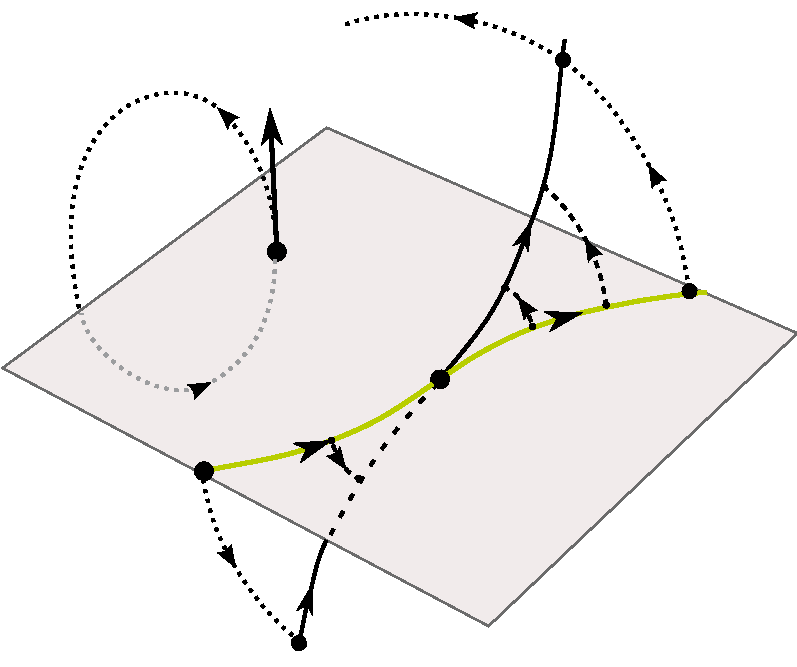
\includegraphics[width=\unitlength]{ReducTraj5.pdf}}%
    \put(0.09054399,0.38282057){\color[rgb]{0,0,0}\rotatebox{-30.34758661}{\makebox(0,0)[lb]{\smash{M}}}}%
    \put(0.57768586,0.29773425){\color[rgb]{0,0,0}\rotatebox{0.0313674}{\makebox(0,0)[lb]{\smash{y(0)}}}}%
    \put(0.59310014,0.69932675){\color[rgb]{0,0,0}\rotatebox{0.03136739}{\makebox(0,0)[lb]{\smash{x(τ)}}}}%
    \put(0.8268425,0.39772328){\color[rgb]{0,0,0}\rotatebox{0.03136739}{\makebox(0,0)[lb]{\smash{y(τ)}}}}%
    \put(0.81220962,0.66529577){\color[rgb]{0,0,0}\rotatebox{0.03136739}{\makebox(0,0)[lb]{\smash{g(τ)}}}}%
    \put(0.23150193,0.63610779){\color[rgb]{0,0,0}\rotatebox{0.0313674}{\makebox(0,0)[lb]{\smash{g}}}}%
    \put(0.37740434,0.49597258){\color[rgb]{0,0,0}\rotatebox{0.0313674}{\makebox(0,0)[lb]{\smash{y'}}}}%
    \put(0.3627714,0.69665188){\color[rgb]{0,0,0}\rotatebox{0.0313674}{\makebox(0,0)[lb]{\smash{t'}}}}%
  \end{picture}%
\endgroup
